\chapter{Používanie aplikácie}

\label{kap:pouzivanie}

\section{Úvodná strana a bodová mapa}

Aplikáciu je možné používať na adrese \href{adresa}{text}. Po otvorení aplikácie sa ako prvá zobrazí stránka obahujúca nástroje na 
zobrazovanie mapy sveta s bodmi označujúcimi IP adresy zoskupené podľa lokality. Vo vrchnej časti aplikácie sa nachádza menu pomocou 
ktorého je možné prechádzať medzi podstránkami aplikácie. Pod ním sa nachádza nadpis popisujúci dané zobrazenie. Vľavo pod nadpisom je umiestnený 
selektor týždňov, pomocou ktorého je možné určiť týždeň, pre ktorý chceme dáta zobraziť. Po zmene hodnoty v selektore sa dáta zmenia okamžite. 
Prednastavená hodnota pri zobrazení aplikácie je posledný týždeň, pre ktorý existujú spracované dáta. V hlavnej sekcii aplikácie vidíme samotné 
zobrazenie dát pomocou mapy. V mape v ľavo dole sa tiež nachádza legenda, ktorá bližšie opisuje koľko konkrétne IP adries je znázornených kruhom 
určenej veľkosti a aká priemerná doba odozvy príkazu ping je zobrazená danou farbou. Detaily výpočtu sú opísané v kapitole \ref{postupy}. 

\begin{figure}
    \centerline{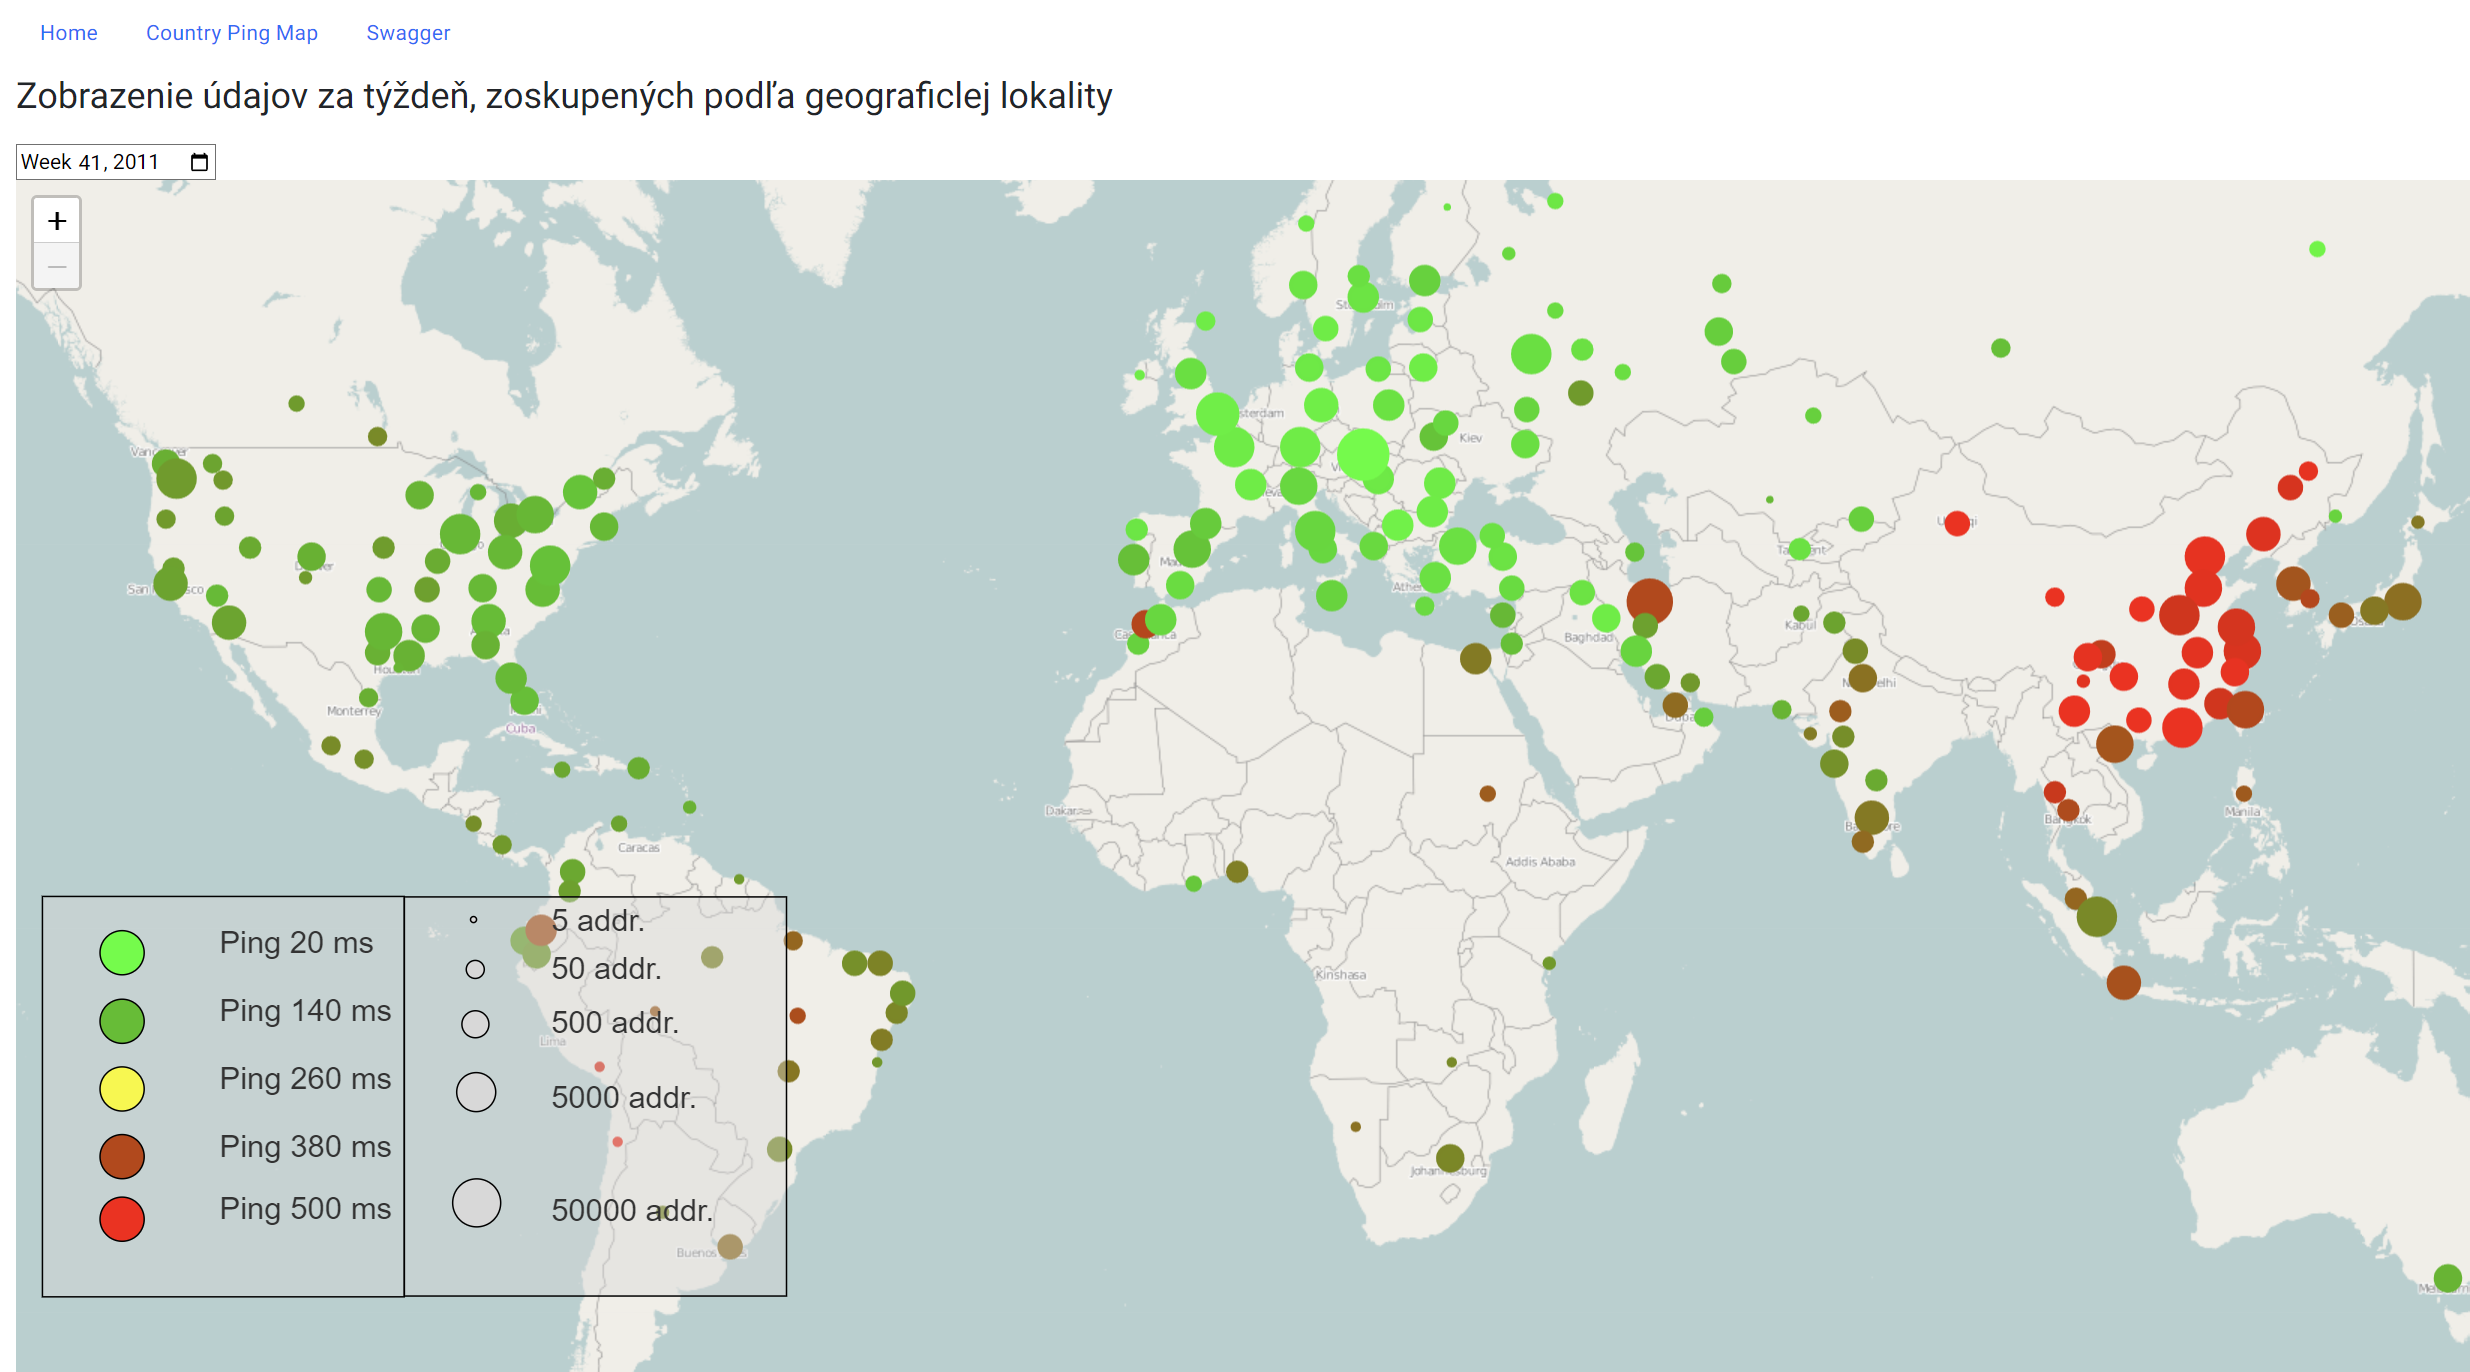
\includegraphics[width=0.8\textwidth]{images/map-points}}
    %popis obrazku
    \caption[Úvodná strana s mapou]{Na úvodnej stránke aplikácie vidíme menu, pod ním nadpis a selektor týždňa. Nakoniec vidíme mapu s bodmi 
    znázorňujúcimi IP adresy ktoré úspešne odpovedali na ping v danom týždni zoskupené podľa lokality. V ľavo dole je legenda znázorňujúca prevod veľkosti
    kruhu na počet IP adries a farby kruhu na ping v milisekundách.}
    %id obrazku, pomocou ktoreho sa budeme na obrazok odvolavat
    \label{obr:map-points}
\end{figure}

\section{Mapa krajín zafarbených podľa doby trvania odozvy}

Po kliknutí na podstránku Country Ping Map sa zobrazí mapa sveta s krajinami zafarbenými podľa priemernej doby pingu pre zvolený týždeň. Vo vrchnej časti 
zostalo nezmeneené menu a rovnako aj selektor týždňov. Vedľa selektora pribudol prepínač škály. Ten rozhoduje, či je pre maximálnu hodnotu použitá hodnota 
500 milisekúnd a všetko ostatné už je len rovnako červené, alebo je ako maximum použitá maximálna hodnota z daného týždňa. Po prepnutí prepínača sa mapa 
prekreslí okamžite, rovnako ako po prepnutí týždňa. V hlavnej časti sa nachádza samotná mapa s legendou, tentoraz opisujúcov len prevod farieb na konkrétnu 
dobu odozvy. Po prejdení myšou nad krajinu sa zobrazí okno s názvom krajiny a konkrétnou hodnotou doby odozvy.
\begin{figure}
    \centerline{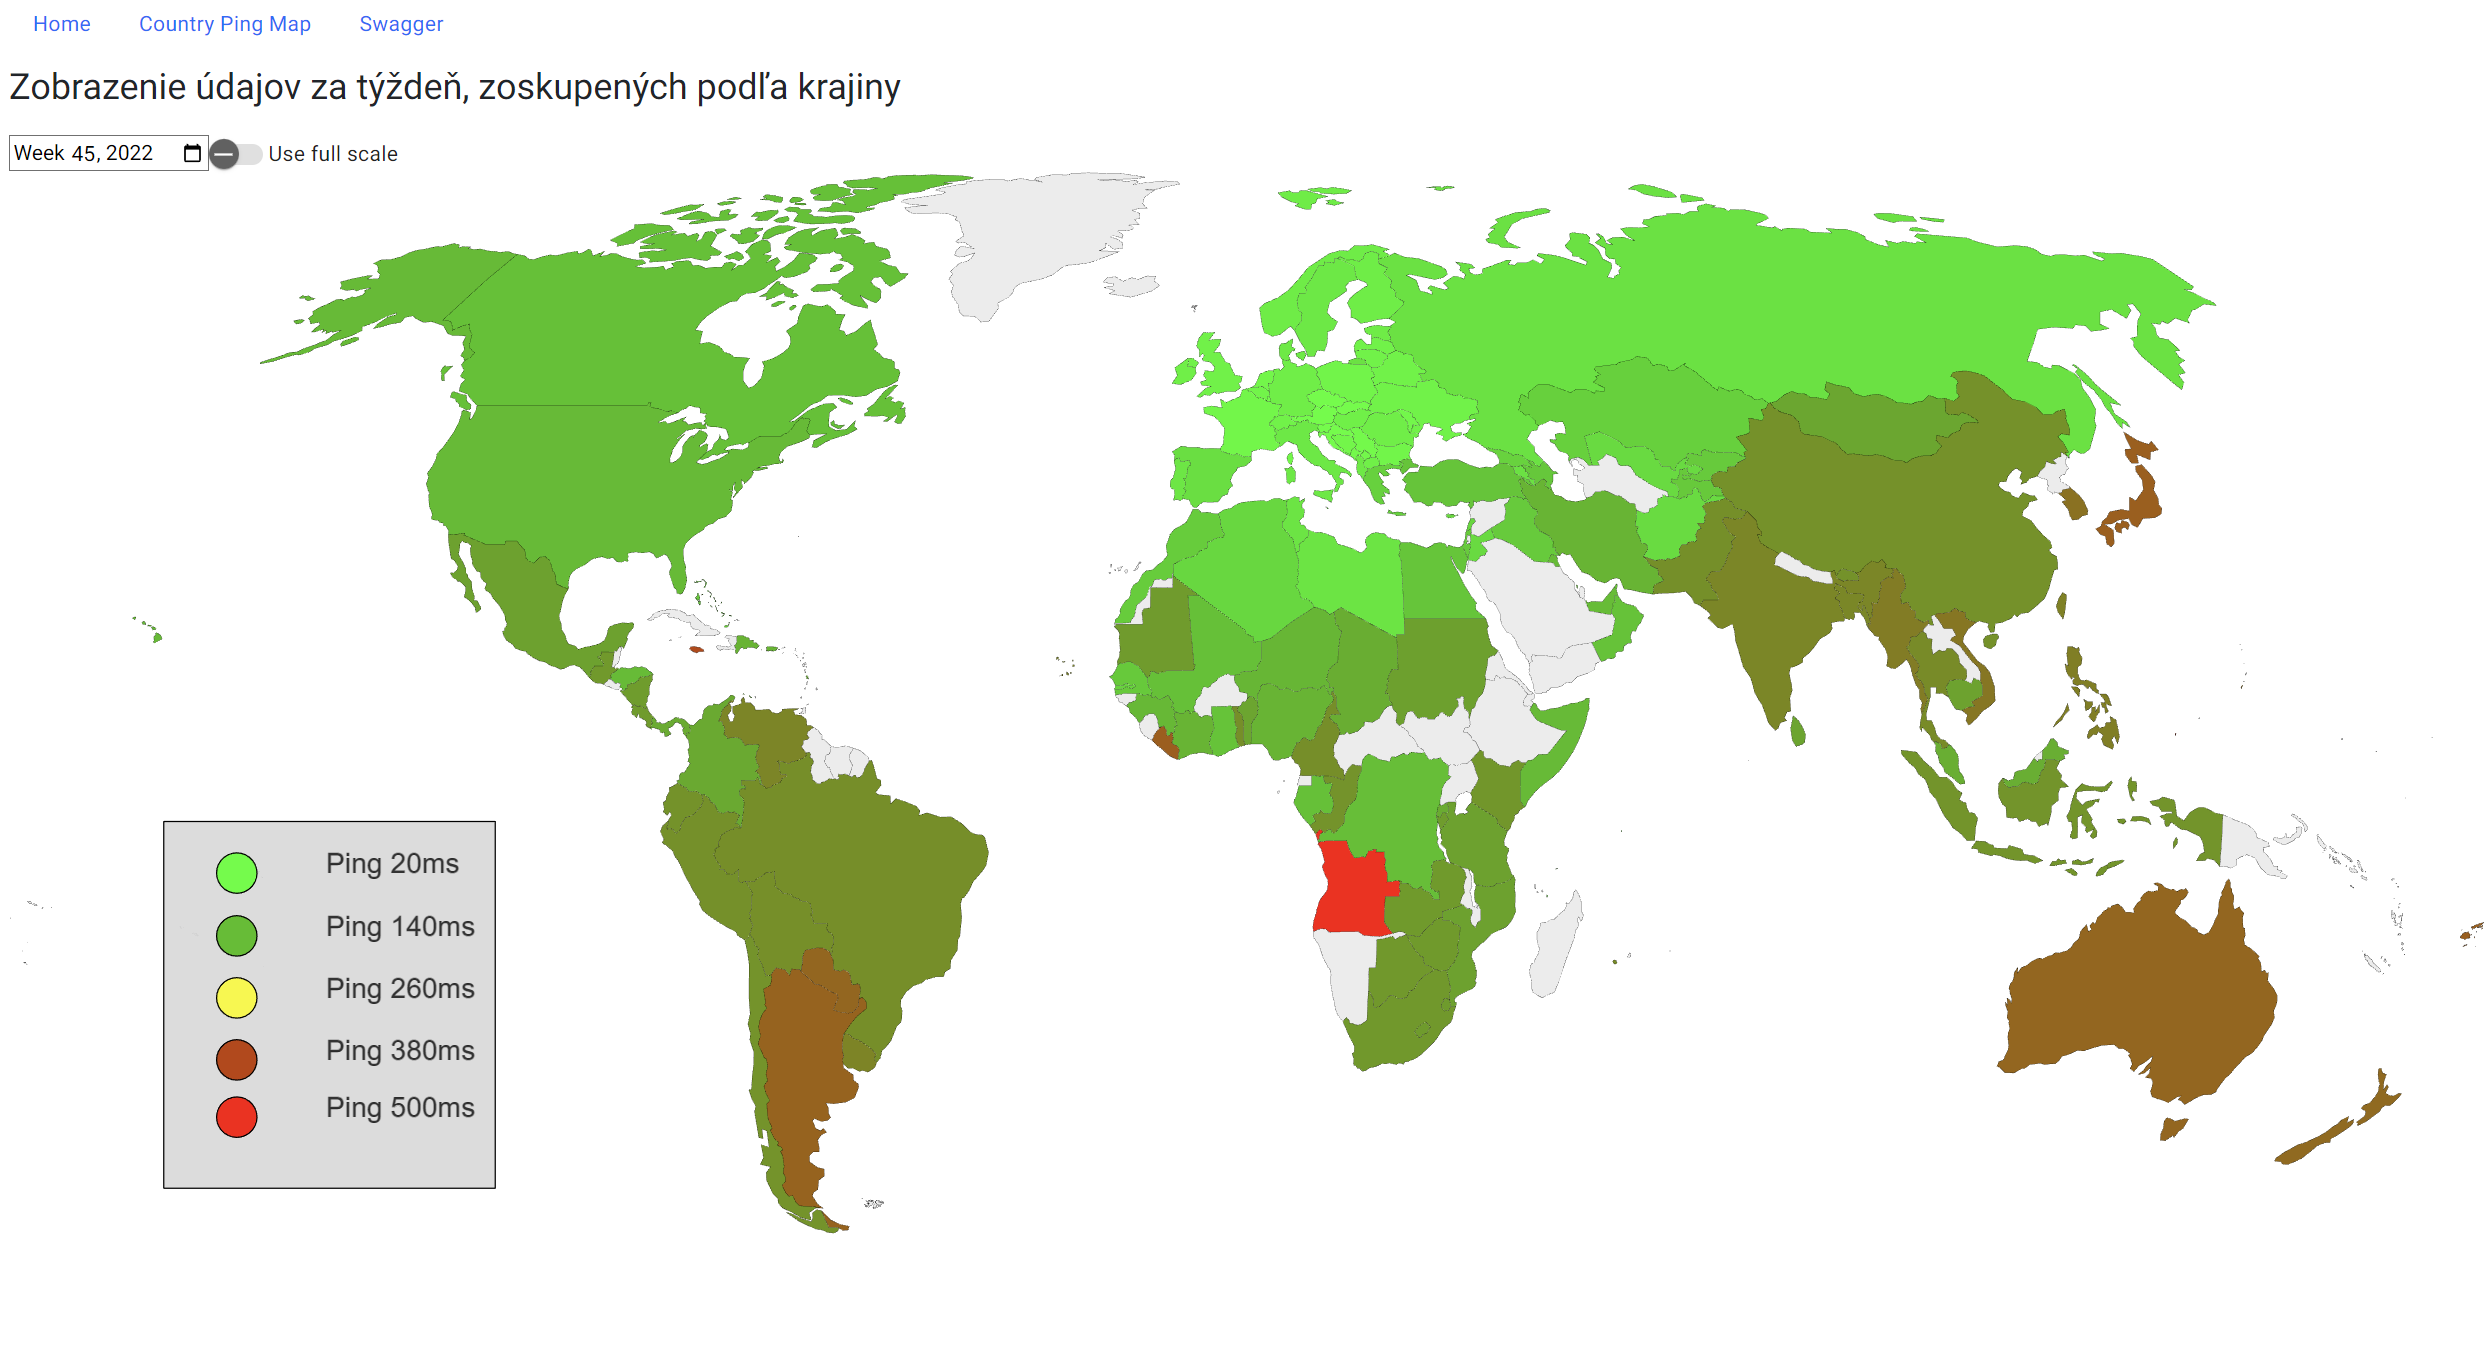
\includegraphics[width=0.8\textwidth]{images/country-ping-info}}
    %popis obrazku
    \caption[Mapa krajín zafarbených podľa priemernej doby odozvy]{Na podstránke je vidno hlavné menu, taktiež pod ním selektor týždňov a samotnú mapu. Oproti 
    domovskej stránke pribudol prepínač škály. }
    %id obrazku, pomocou ktoreho sa budeme na obrazok odvolavat
    \label{obr:country-ping-info}
\end{figure}